% !Mode:: "TeX:UTF-8"
\documentclass[12pt,a4paper]{article}

%%%%%%%%------------------------------------------------------------------------
%%%% 日常所用宏包

%% 控制页边距
% 如果是beamer文档类, 则不用geometry
\makeatletter
\@ifclassloaded{beamer}{}{\usepackage[top=2.5cm, bottom=2.5cm, left=2.5cm, right=2.5cm]{geometry}}
\makeatother

%% 控制项目列表
\usepackage{enumerate}

%% 多栏显示
\usepackage{multicol}

%% 算法环境
\usepackage{algorithm}  
\usepackage{algorithmic} 
\usepackage{float} 

%% 网址引用
\usepackage{url}

%% 控制矩阵行距
\renewcommand\arraystretch{1.4}

%% hyperref宏包,生成可定位点击的超链接,并且会生成pdf书签
\makeatletter
\@ifclassloaded{beamer}{
\usepackage{hyperref}
\usepackage{ragged2e} % 对齐
}{
\usepackage[%
    pdfstartview=FitH,%
    CJKbookmarks=true,%
    bookmarks=true,%
    bookmarksnumbered=true,%
    bookmarksopen=true,%
    colorlinks=true,%
    citecolor=blue,%
    linkcolor=blue,%
    anchorcolor=green,%
    urlcolor=blue%
]{hyperref}
}
\makeatother



\makeatletter % 如果是 beamer 不需要下面两个包
\@ifclassloaded{beamer}{
\mode<presentation>
{
} 
}{
%% 控制标题
\usepackage{titlesec}
%% 控制目录
\usepackage{titletoc}
}
\makeatother

%% 控制表格样式
\usepackage{booktabs}

%% 控制字体大小
\usepackage{type1cm}

%% 首行缩进,用\noindent取消某段缩进
\usepackage{indentfirst}

%%边框
\usepackage{listings}

%% 支持彩色文本、底色、文本框等
\usepackage{color,xcolor}

%% AMS LaTeX宏包: http://zzg34b.w3.c361.com/package/maths.htm#amssymb
\usepackage{amsmath,amssymb}
%% 多个图形并排
\usepackage{subfig}
%%%% 基本插图方法
%% 图形宏包
\usepackage{graphicx}
\newcommand{\red}[1]{\textcolor{red}{#1}}
\newcommand{\blue}[1]{\structure{#1}}
\newcommand{\brown}[1]{\textcolor{brown}{#1}}
\newcommand{\green}[1]{\textcolor{green}{#1}}


%%%% 基本插图方法结束

%%%% pgf/tikz绘图宏包设置
\usepackage{pgf,tikz}
\usetikzlibrary{shapes,automata,snakes,backgrounds,arrows}
\usetikzlibrary{mindmap}
%% 可以直接在latex文档中使用graphviz/dot语言,
%% 也可以用dot2tex工具将dot文件转换成tex文件再include进来
%% \usepackage[shell,pgf,outputdir={docgraphs/}]{dot2texi}
%%%% pgf/tikz设置结束


\makeatletter % 如果是 beamer 不需要下面两个包
\@ifclassloaded{beamer}{

}{
%%%% fancyhdr设置页眉页脚
%% 页眉页脚宏包
\usepackage{fancyhdr}
%% 页眉页脚风格
\pagestyle{plain}
}

%% 有时会出现\headheight too small的warning
\setlength{\headheight}{15pt}

%% 清空当前页眉页脚的默认设置
%\fancyhf{}
%%%% fancyhdr设置结束


\makeatletter % 对 beamer 要重新设置
\@ifclassloaded{beamer}{

}{
%%%% 设置listings宏包用来粘贴源代码
%% 方便粘贴源代码,部分代码高亮功能
\usepackage{listings}

%% 设置listings宏包的一些全局样式
%% 参考http://hi.baidu.com/shawpinlee/blog/item/9ec431cbae28e41cbe09e6e4.html
\lstset{
showstringspaces=false,              %% 设定是否显示代码之间的空格符号
numbers=left,                        %% 在左边显示行号
numberstyle=\tiny,                   %% 设定行号字体的大小
basicstyle=\footnotesize,                    %% 设定字体大小\tiny, \small, \Large等等
keywordstyle=\color{blue!70}, commentstyle=\color{red!50!green!50!blue!50},
                                     %% 关键字高亮
frame=shadowbox,                     %% 给代码加框
rulesepcolor=\color{red!20!green!20!blue!20},
escapechar=`,                        %% 中文逃逸字符,用于中英混排
xleftmargin=2em,xrightmargin=2em, aboveskip=1em,
breaklines,                          %% 这条命令可以让LaTeX自动将长的代码行换行排版
extendedchars=false                  %% 这一条命令可以解决代码跨页时,章节标题,页眉等汉字不显示的问题
}}
\makeatother
%%%% listings宏包设置结束


%%%% 附录设置
\makeatletter % 对 beamer 要重新设置
\@ifclassloaded{beamer}{

}{
\usepackage[title,titletoc,header]{appendix}
}
\makeatother
%%%% 附录设置结束


%%%% 日常宏包设置结束
%%%%%%%%------------------------------------------------------------------------


%%%%%%%%------------------------------------------------------------------------
%%%% 英文字体设置结束
%% 这里可以加入自己的英文字体设置
%%%%%%%%------------------------------------------------------------------------

%%%%%%%%------------------------------------------------------------------------
%%%% 设置常用字体字号,与MS Word相对应

%% 一号, 1.4倍行距
\newcommand{\yihao}{\fontsize{26pt}{36pt}\selectfont}
%% 二号, 1.25倍行距
\newcommand{\erhao}{\fontsize{22pt}{28pt}\selectfont}
%% 小二, 单倍行距
\newcommand{\xiaoer}{\fontsize{18pt}{18pt}\selectfont}
%% 三号, 1.5倍行距
\newcommand{\sanhao}{\fontsize{16pt}{24pt}\selectfont}
%% 小三, 1.5倍行距
\newcommand{\xiaosan}{\fontsize{15pt}{22pt}\selectfont}
%% 四号, 1.5倍行距
\newcommand{\sihao}{\fontsize{14pt}{21pt}\selectfont}
%% 半四, 1.5倍行距
\newcommand{\bansi}{\fontsize{13pt}{19.5pt}\selectfont}
%% 小四, 1.5倍行距
\newcommand{\xiaosi}{\fontsize{12pt}{18pt}\selectfont}
%% 大五, 单倍行距
\newcommand{\dawu}{\fontsize{11pt}{11pt}\selectfont}
%% 五号, 单倍行距
\newcommand{\wuhao}{\fontsize{10.5pt}{10.5pt}\selectfont}
%%%%%%%%------------------------------------------------------------------------


%% 设定段间距
\setlength{\parskip}{0.5\baselineskip}

%% 设定行距
\linespread{1}


%% 设定正文字体大小
% \renewcommand{\normalsize}{\sihao}

%制作水印
\RequirePackage{draftcopy}
\draftcopyName{XTUMESH}{100}
\draftcopySetGrey{0.90}
\draftcopyPageTransform{40 rotate}
\draftcopyPageX{350}
\draftcopyPageY{80}

%%%% 个性设置结束
%%%%%%%%------------------------------------------------------------------------


%%%%%%%%------------------------------------------------------------------------
%%%% bibtex设置

%% 设定参考文献显示风格
% 下面是几种常见的样式
% * plain: 按字母的顺序排列,比较次序为作者、年度和标题
% * unsrt: 样式同plain,只是按照引用的先后排序
% * alpha: 用作者名首字母+年份后两位作标号,以字母顺序排序
% * abbrv: 类似plain,将月份全拼改为缩写,更显紧凑
% * apalike: 美国心理学学会期刊样式, 引用样式 [Tailper and Zang, 2006]

\makeatletter
\@ifclassloaded{beamer}{
\bibliographystyle{apalike}
}{
\bibliographystyle{unsrt}
}
\makeatother


%%%% bibtex设置结束
%%%%%%%%------------------------------------------------------------------------

%%%%%%%%------------------------------------------------------------------------
%%%% xeCJK相关宏包

\usepackage{xltxtra,fontspec,xunicode}
\usepackage[slantfont, boldfont]{xeCJK} 

\setlength{\parindent}{2em}%中文缩进两个汉字位

%% 针对中文进行断行
\XeTeXlinebreaklocale "zh"             

%% 给予TeX断行一定自由度
\XeTeXlinebreakskip = 0pt plus 1pt minus 0.1pt

%%%% xeCJK设置结束                                       
%%%%%%%%------------------------------------------------------------------------
\usepackage{ listings} 
\usepackage{ xcolor}
%%%%%%%%------------------------------------------------------------------------
%%%% xeCJK字体设置

%% 设置中文标点样式,支持quanjiao、banjiao、kaiming等多种方式
\punctstyle{kaiming}                                        
\usepackage{framed}%%边框                                                
%% 设置缺省中文字体
%\setCJKmainfont[BoldFont={Adobe Heiti Std}, ItalicFont={Adobe Kaiti Std}]{Adobe Song Std}   
\setCJKmainfont{SimSun}
%% 设置中文无衬线字体
%\setCJKsansfont[BoldFont={Adobe Heiti Std}]{Adobe Kaiti Std}  
%% 设置等宽字体
%\setCJKmonofont{Adobe Heiti Std}                            

%% 英文衬线字体
\setmainfont{DejaVu Serif}                                  
%% 英文等宽字体
\setmonofont{DejaVu Sans Mono}                              
%% 英文无衬线字体
\setsansfont{DejaVu Sans}                                   

%% 定义新字体
\setCJKfamilyfont{song}{Adobe Song Std}                     
\setCJKfamilyfont{kai}{Adobe Kaiti Std}
\setCJKfamilyfont{hei}{Adobe Heiti Std}
\setCJKfamilyfont{fangsong}{Adobe Fangsong Std}
\setCJKfamilyfont{lisu}{LiSu}
\setCJKfamilyfont{youyuan}{YouYuan}

%% 自定义宋体
\newcommand{\song}{\CJKfamily{song}}                       
%% 自定义楷体
\newcommand{\kai}{\CJKfamily{kai}}                         
%% 自定义黑体
\newcommand{\hei}{\CJKfamily{hei}}                         
%% 自定义仿宋体
\newcommand{\fangsong}{\CJKfamily{fangsong}}               
%% 自定义隶书
\newcommand{\lisu}{\CJKfamily{lisu}}                       
%% 自定义幼圆
\newcommand{\youyuan}{\CJKfamily{youyuan}}                 

%%%% xeCJK字体设置结束
%%%%%%%%------------------------------------------------------------------------

%%%%%%%%------------------------------------------------------------------------
%%%% 一些关于中文文档的重定义
\newcommand{\chntoday}{\number\year\,年\,\number\month\,月\,\number\day\,日}
%% 数学公式定理的重定义

%% 中文破折号,据说来自清华模板
\newcommand{\pozhehao}{\kern0.3ex\rule[0.8ex]{2em}{0.1ex}\kern0.3ex}

\newtheorem{example}{例}                                   
\newtheorem{theorem}{定理}[section]                         
\newtheorem{definition}{定义}
\newtheorem{axiom}{公理}
\newtheorem{property}{性质}
\newtheorem{proposition}{命题}
\newtheorem{lemma}{引理}
\newtheorem{corollary}{推论}
\newtheorem{remark}{注解}
\newtheorem{condition}{条件}
\newtheorem{conclusion}{结论}
\newtheorem{assumption}{假设}

\makeatletter %
\@ifclassloaded{beamer}{

}{
%% 章节等名称重定义
\renewcommand{\contentsname}{目录}     
\renewcommand{\indexname}{索引}
\renewcommand{\listfigurename}{插图目录}
\renewcommand{\listtablename}{表格目录}
\renewcommand{\appendixname}{附录}
\renewcommand{\appendixpagename}{附录}
\renewcommand{\appendixtocname}{附录}
%% 设置chapter、section与subsection的格式
\titleformat{\chapter}{\centering\huge}{第\thechapter{}章}{1em}{\textbf}
\titleformat{\section}{\centering\sihao}{\thesection}{1em}{\textbf}
\titleformat{\subsection}{\xiaosi}{\thesubsection}{1em}{\textbf}
\titleformat{\subsubsection}{\xiaosi}{\thesubsubsection}{1em}{\textbf}

\@ifclassloaded{book}{

}{
\renewcommand{\abstractname}{摘要}
}
}
\makeatother

\renewcommand{\figurename}{图}
\renewcommand{\tablename}{表}

\makeatletter
\@ifclassloaded{book}{
\renewcommand{\bibname}{参考文献}
}{
\renewcommand{\refname}{参考文献} 
}
\makeatother

\floatname{algorithm}{算法}
\renewcommand{\algorithmicrequire}{\textbf{输入:}}
\renewcommand{\algorithmicensure}{\textbf{输出:}}

%%%% 中文重定义结束
%%%%%%%%------------------------------------------------------------------------


\title{非对称特征值问题}
\begin{document}
\maketitle
\noindent \textbf{非对称矩阵特征值/特征向量的计算}\\
基本约定1:$A \in \mathbb{R}^{n \times n}$、非对称、稠密\\
基本约定2:~$\left|\lambda_{1}\right| \geq\left|\lambda_{2}\right| \geq \cdots \geq\left|\lambda_{n}\right| \geq 0$\\
\\
本讲主要讨论如何计算 A 的\textcolor{blue}{全部特征值和/或特征向量}\\
主要介绍以下方法:\\
\begin{itemize}
\item 幂迭代方法
\item  反迭代方法(位移策略,Rayleigh 商迭代) \item 正交迭代方法
\item QR方法
\end{itemize}
关于稠密矩阵特征值计算的参考资料有:\\
\begin{itemize}
\item J.H.Wilkinson,TheAlgebraicEigenvalueProblem,1965
\item B.N.Parlett,TheSymmetricEigenvalueProblem,2ndEds.,1998
\item G.W.Stewart,MatrixAlgorithms,VolII:Eigensystems,2001
\item G.H.GolubandC.F.VanLoan,MatrixComputations,2013
\item P.Arbenz,Thecourse252-0504-00G,
\end{itemize}
\textcolor{blue}{Numerical Methods for Solving Large Scale Eigenvalue Problems, 2018.
(该课程的主页)}
\section{幂迭代}
\textcolor{blue}{幂迭代} 是计算特征值和特征向量的一种简单易用的算法.\\
虽然简单, 但它却建立了计算特征值和特征向量的算法的一个基本框架.\\
\textcolor{blue}{算法 1.1} 幂迭代算法 (Power Iteration)
\begin{enumerate}[1:]
\item Choose an initial guess $x(0)$ with $||x(0)||_{2} = 1$
\item set $k=0$
\item while not convergence do
\item \qquad$y^{(k+1)} = Ax^{(k)}$
\item \qquad$x^{(k+1)}=y^{(k+1)} /\left\|y^{(k+1)}\right\|_{2}$
\item \qquad$\mu_{k+1}=\left(x^{(k+1)}, A x^{(k+1)}\right)$
\item \qquad$k=k+1$
\item end while
\end{enumerate}
 幂迭代的收敛性\\
 假设1:$A \in \mathbb{R}^{n \times n}$可对角化,即$A=V \Lambda V^{-1}$,其中
$$
\Lambda=\operatorname{diag}\left(\lambda_{1}, \ldots, \lambda_{n}\right), \quad V=\left[v_{1}, \ldots, v_{n}\right] \in \mathbb{C}^{n \times n}, \quad\left\|v_{i}\right\|_{2}=1
$$
假设2:$\left|\lambda_{1}\right|>\left|\lambda_{2}\right| \geq\left|\lambda_{3}\right| \geq \cdots \geq\left|\lambda_{n}\right|$
由于 V 的列向量组构成$\mathbb{C}^{n}$的一组基, 因此$x^{(0)}$可表示为
$$
x^{(0)}=\alpha_{1} v_{1}+\alpha_{2} v_{2}+\cdots+\alpha_{n} v_{n}=V\left[\alpha_{1}, \alpha_{2}, \ldots, \alpha_{n}\right]^{\top}
$$
我们假定$\alpha_{1} \neq 0$,即$x^{(0)}$不属于$\operatorname{span}\left\{v_{2}, v_{3}, \ldots, v_{n}\right\}$
(由于$x^{(0)}$) 是随机选取的, 从概率意义上讲, 这个假设通常是成立的).\\
于是我们可得
$$
A^{k} x^{(0)}=\left(V \Lambda V^{-1}\right)^{k} V\left[\begin{array}{c}{\alpha_{1}} \\ {\alpha_{2}} \\ {\vdots} \\ {\alpha_{n}}\end{array}\right]=V \Lambda^{k}\left[\begin{array}{c}{\alpha_{1}} \\ {\alpha_{2}} \\ {\vdots} \\ {\alpha_{n}}\end{array}\right]=V\left[\begin{array}{c}{\alpha_{1} \lambda_{1}^{k}} \\ {\alpha_{2} \lambda_{2}^{k}} \\ {\vdots} \\ {\alpha_{n} \lambda_{n}^{k}}\end{array}\right]
$$
$$
=\alpha_{1} \lambda_{1}^{k} V\left[\begin{array}{c}{1} \\ {\frac{\alpha_{2}}{\alpha_{1}}\left(\frac{\lambda_{2}}{\lambda_{1}}\right)^{k}} \\ {\vdots} \\ {\frac{\alpha_{n}}{\alpha_{1}}\left(\frac{\lambda_{n}}{\lambda_{1}}\right)^{k}}\end{array}\right]
$$
又$\left|\lambda_{i} / \lambda_{1}\right|<1, i=2,3, \ldots, n$,所以
$$
\lim _{k \rightarrow \infty}\left(\frac{\lambda_{i}}{\lambda_{1}}\right)^{k}=0, \quad i=2,3, \ldots, n
$$
故当 k 趋向于无穷大时, 向量
$$
\left[1, \frac{\alpha_{2}}{\alpha_{1}}\left(\frac{\lambda_{2}}{\lambda_{1}}\right)^{k}, \ldots, \frac{\alpha_{n}}{\alpha_{1}}\left(\frac{\lambda_{n}}{\lambda_{1}}\right)^{k}\right]^{\top}, \quad k=0,1,2, \ldots
$$
收敛到$e_{1}=[1,0, \ldots, 0]^{\top}$\\
所以向量$x^{(k)}=A^{k} x^{(0)} /\left\|A^{k} x^{(0)}\right\|_{2}$收敛到$\pm v_{1}$,即$\lambda_{1}$的特征向量.而$\mu_{k}=\left(x^{(k)}\right)^{*} A x^{(k)}$则收敛到$v_{1}^{*} A v_{1}=\lambda_{1}$
$\dagger$幂迭代的收敛快慢取决于$\left|\lambda_{2} / \lambda_{1}\right|$的大小,$\left|\lambda_{2} / \lambda_{1}\right|$越小,收敛越快.\\
\begin{itemize}
\item 幂迭代只能用于计算(模)最大的特征值和其相应的特征向量
\item 当$\left|\lambda_{2} / \lambda_{1}\right|$接近于 1 时, 收敛速度会非常慢
\item 如果模最大的特征值是一对共轭复数,则幂迭代可能会失效.
\end{itemize}
加速技巧:位移策略\\
出发点: 加快幂迭代算法的收敛速度$\Longleftrightarrow$尽可能地减小$\left|\lambda_{2} / \lambda_{1}\right|$\\
\textcolor{blue}{位移策略:}计算$A-\sigma I$的特征值\\
我们称$\sigma$为\textcolor{blue}{位移},满足
\begin{enumerate}[(1)]
\item $\lambda_{1}-\sigma$是$A-\sigma I$的模最大特征值
\item $
\max _{2 \leq i \leq n}\left|\frac{\lambda_{i}-\sigma}{\lambda_{1}-\sigma}\right|
$尽可能地小
\end{enumerate}
其中第一个条件保证最后所求得的特征值是我们所要的, 第二个条件用 于加快幂迭代的收敛速度.\\
缺点:(1)$\sigma$很难选取;(2)加速效果有限\\
改进: \textcolor{blue}{与反迭代相结合, 能起到很好的加速效果}
\section{反迭代}
\noindent 用幂迭代求$A^{-1}$的模最小特征值,这就是\textcolor{blue}{反迭代}\\
\textcolor{blue}{算法 2.1} 反迭代算法 (Inverse Iteration)\\
\begin{enumerate}[1:]
\item Choose an initial guess $x(0)$ with $||x(0)||_{2} = 1$
\item set $k=0$
\item while not convergence do
\item \qquad$y^{(k+1)} = (A-\sigma I)^{-1}x^{(k)}$
\item \qquad$x^{(k+1)}=y^{(k+1)} /\left\|y^{(k+1)}\right\|_{2}$
\item \qquad$\mu_{k+1}=\left(x^{(k+1)}, A x^{(k+1)}\right)$
\item \qquad$\sigma=\mu_{k+1},k=k+1$
\item end while
\end{enumerate}
显然:$\mu_{k}$收敛到$\sigma$最近的特征值,$x^({k})$收敛到对应的特征向量\\
$\dagger$\textcolor{blue}{理论上, 反迭代 + 位移策略, 可以计算矩阵的任意一个特征值}\\
优点:
\begin{itemize}
\item 若$\sigma$ 与某个特征值 $\lambda_{k}$ 非常接近, 则反迭代算法的收敛速度非常快
\item 只要选取合适的位移$\sigma$,就可以计算A的任意一个特征值.
\end{itemize}
缺点:
\begin{itemize}
\item 每步迭代需要解一个线性方程组 $(A-\sigma I) y^{(k+1)}=x^{(k)}$这需要对$A-\sigma I$做LU或PLU分解
\item 与幂迭代一样,反迭代算法一次只能求一个特征值
\item 怎样选取位移$\sigma ? \rightarrow$ \textcolor{blue}{Rayleigh 商}动态选取, 自动调整
\end{itemize}
\subsection{\textcolor{blue}{Rayleigh 商迭代}}
\noindent \textcolor{blue}{出发点}:使得 $\sigma$ 与所求的特征值越靠近越好.\\
\\
\textcolor{blue}{期望能直接给出一个理想位移是不太现实的. 比较现实的方法就是动态 调整, 使得位移逐渐靠近某个特征值.}\\
Rayleigh 商迭代: \textcolor{blue}{以 Rayleigh 商 $\mu_{k}$为第 k 步的位移}\\
 理由:$\mu_{k}$ 会逐渐收敛到某个特征值.\\
 \\
\textcolor{blue}{算法 2.2} Rayleigh 商迭代 (Rayleigh Quotient Iteration, RQI)\\
\begin{enumerate}
\item Choose an initial vector $x(0)$ with $||x(0)||_{2} = 1$
\item set $k=0$
\item compute $\sigma=\left(x^{(0)}\right)^{*} A x^{(0)}$
\item while not convergence do
\item \qquad$y^{(k+1)} = (A-\sigma I)^{-1}x^{(k)}$
\item \qquad$x^{(k+1)}=y^{(k+1)} /\left\|y^{(k+1)}\right\|_{2}$
\item \qquad$\mu_{k+1}=\left(x^{(k+1)}, A x^{(k+1)}\right)$
\item \qquad$\sigma=\mu_{k+1}$
\item \qquad$k=k+1$
\item end while
\end{enumerate}
 RQI 算法的收敛性\\
 \\
 一般来说, 如果 Rayleigh 商迭代收敛到 A 的一个单特征值, 则至少是二 次收敛的, 即具有局部二次收敛性. 如果 A 是对称的, 则能达到局部三 次收敛, 详情见后面的\textcolor{blue}{对称特征值问题.}\\
 \\
 缺点:\\
由于每次迭代的位移是不同的, 因此每次迭代需要求解一个不同的线性方程组, 这使得运算量大大增加. \\
因此通常应用于 \textcolor{blue}{三对角矩阵} 的特征值计算
\section{正交迭代}
\noindent 出发点:同时计算多个特征值/特征向量\\
策略: 同时采用多个初始向量, 希望收敛到 A 的一个不变子空间\\
\textcolor{blue}{算法 3.1} 正交迭代算法 (Orthogonal Iteration)\\
\begin{enumerate}[1:]
\item Choose an initial vector$n\times p$column orthogonal matrix $Z_{0}$ 
\item set $k=0$
\item while not convergence do
\item \qquad compute $Y^{(k+1)} = AZ_{(k)}$
\item \qquad$Y_{(k+1)}=Z_{(k+1)}\hat{R}_{k+1}$
\item \qquad$k=k+1$
\item end while
\end{enumerate}
\textcolor{blue}{说明}:\\
在算法中使用 QR 分解是为了保持$z_k$的列正交性, 使得其列向量组构 成子空间 span$\{A^kZ_0\}$的一组正交基. 一方面提高算法的数值稳定性, 另一方面避免所有列都收敛到最大特征值所对应的特征向量.\\
收敛性分析\\
假设 A 是可对角化的, 即$A=V \Lambda V^{-1}$,其中$\Lambda=\operatorname{diag}\left(\lambda_{1}, \lambda_{2}, \ldots, \lambda_{n}\right)$,且$\left|\lambda_{1}\right| \geq \cdots \geq\left|\lambda_{p}\right|>\left|\lambda_{p+1}\right| \geq \cdots \geq\left|\lambda_{n}\right|$.则可得
$$
\operatorname{span}\left\{Z_{k}\right\}=\operatorname{span}\left\{Y_{k}\right\}=\operatorname{span}\left\{A Z_{k-1}\right\}, \quad k=1,2, \ldots
$$
由此可知
$$
\operatorname{span}\left\{Z_{k}\right\}=\operatorname{span}\left\{A^{k} Z_{0}\right\}=\operatorname{span}\left\{V \Lambda^{k} V^{-1} Z_{0}\right\}
$$
我们注意到
$$
\Lambda^{k} V^{-1} Z_{0}=\lambda_{p}^{k}\left[\begin{array}{ccccc}
{\left(\lambda_{1} / \lambda_{p}\right)^{k}} & {} & {} &{}&{}\\ 
{} & {\ddots} & {} & {} &{}\\
 {} & {} & {1}& {} & {} \\ 
{} & {} & {} & {\ddots} & {} \\
 {} & {} & {} & {} & {\left(\lambda_{n} / \lambda_{p}\right)^{k}}
 \end{array}\right]V^{-1} Z_{0} \triangleq \lambda_{p}^{k}\left[\begin{array}{c}
 {W_{p}^{(k)}} \\ 
 {W_{n-p}^{(k)}}
 \end{array}\right]
$$
由于当$i>p$时有$\left|\lambda_{i} / \lambda_{p}\right|<1$,所以当k趋于无穷大时,
$W_{n-p}^{(k)}$趋向于0,令$V=\left[V_{p}, V_{n-p}\right]$,则
$$V \Lambda^{k} V^{-1} Z_{0}=\lambda_{p}^{k}\left[V_{p}, V_{n-p}\right]\left[\begin{array}{c}{W_{p}^{(k)}} \\ {W_{n-p}^{(k)}}\end{array}\right]=\lambda_{p}^{k}\left(V_{p} W_{p}^{(k)}+V_{n-p} W_{n-p}^{(k)}\right)$$
所以当$k \rightarrow \infty$时,有
$$
\begin{aligned} \operatorname{span}\left\{Z_{k}\right\}=\operatorname{span}\left\{V \Lambda^{k} V^{-1} Z_{0}\right\} &=\operatorname{span}\left\{V_{p} W_{p}^{(k)}+V_{n-p} W_{n-p}^{(k)}\right\} \\ & \rightarrow \operatorname{span}\left\{V_{p} W_{p}^{(k)}\right\}=\operatorname{span}\left\{V_{p}\right\} \end{aligned}
$$
即$\operatorname{span}\left\{Z_{k}\right\}$趋向于 A 的一个 $p$ 维不变子空间$\operatorname{span}\left\{V_{p}\right\}$\\
\\
\textcolor{blue}{定理}~~给定正整数$p(1 \leq p \leq n)$,考虑算法3.1,假设A是可对角化的,且$\left|\lambda_{1}\right| \geq \cdots \geq\left|\lambda_{p}\right|>\left|\lambda_{p+1}\right| \geq \cdots \geq\left|\lambda_{n}\right|$.则
$\operatorname{span}\left\{Z_{k}\right\}$收敛到A的一 个 $p$ 维不变子空间.\\
\textcolor{blue}{说明:}\\
如果 A 不可对角化, 利用 Jordan 标准型, 可以到同样的结论, 见 \textcolor{blue}{[Watkins 2007, Watkins-Elsner 1991]}.\\
$\dagger$在正交迭代中, 如果我们取 $Z_{0} = I$, 则可得到一类特殊的正交迭代算 法. 此时, 在一定条件下, 正交迭代会收敛到 $A$ 的 Schur 标准型.
\section{QR迭代}
\begin{enumerate}[4.1]
\item 算法介绍
\item  QR 迭代与幂迭代的关系
\item  QR 迭代与反迭代的关系
\item  QR 迭代与正交迭代的关系
\item  QR 迭代的收敛性
\item  带位移的 QR 迭代
\end{enumerate}
\subsection{算法介绍}
\noindent \textcolor{blue}{基本思想}:通过不断的正交相似变换, 将 A 转化为 (拟) 上三角形式\\
\textcolor{blue}{算法 4.1} QR 迭代算法 (QR Iteration)\\
\begin{enumerate}[1:]
\item Set $A_{1}=A$ and $k=1$
\item while not convergence do
\item \qquad $[Q_{k},R_{k}]=qr(A_{k})$
\item \qquad compute $A_{k+1}=R_{k}Q_{k}$
\item \qquad$k=k+1$
\item end while
\end{enumerate}
正交相似性
在 QR 迭代算法中, 我们有
$$
A_{k+1}=R_{k} Q_{k}=\left(Q_{k}^{\top} Q_{k}\right) R_{k} Q_{k}=Q_{k}^{\top}\left(Q_{k} R_{k}\right) Q_{k}=Q_{k}^{\top} A_{k} Q_{k}
$$
由这个递推关系可得
$$
A_{k+1}=Q_{k}^{\top} A_{k} Q_{k}=\cdots=Q_{k}^{\top} Q_{k-1}^{\top} \cdots Q_{1}^{\top} A Q_{1} \cdots Q_{k-1} Q_{k}
$$
记$\tilde{Q}_{k}=Q_{1} \cdots Q_{k-1} Q_{k}$=$\left[\begin{array}{ll}{\tilde{q}_{1}^{(k)},} & {\tilde{q}_{2}^{(k)}, \ldots, \tilde{q}_{n}^{(k)}}\end{array}\right]$
则
\begin{equation} 
A_{k+1}=\tilde{Q}_{k}^{\top} A \tilde{Q}_{k}
\end{equation}
即$A_{k+1}$与$A$正交相似
\subsection{\textcolor{blue}{QR 迭代与幂迭代的关系}}
记$\tilde{R}_{k}=R_{k} R_{k-1} \cdots R_{1}$,则有
$$
\begin{aligned} 
\tilde{Q}_{k} \tilde{R}_{k} &=\tilde{Q}_{k-1}\left(Q_{k} R_{k}\right) \tilde{R}_{k-1}=\tilde{Q}_{k-1}\left(A_{k}\right) \tilde{R}_{k-1} \\ 
&=\tilde{Q}_{k-1}\left(\tilde{Q}_{k-1}^{\top} A \tilde{Q}_{k-1}\right) \tilde{R}_{k-1} \\ 
&=A \tilde{Q}_{k-1} \tilde{R}_{k-1} 
\end{aligned}
$$
由此递推下去, 即可得
$$
\tilde{Q}_{k} \tilde{R}_{k}=A^{k-1} \tilde{Q}_{1} \tilde{R}_{1}=A^{k-1} Q_{1} R_{1}=A^{k}
$$
故
$$
\tilde{Q}_{k} \tilde{R}_{k} e_{1}=A^{k} e_{1}
$$
假设$\left|\lambda_{1}\right|>\left|\lambda_{2}\right| \geq \cdots \geq\left|\lambda_{n}\right|$,则当k充分大时,$A^{k} e_{1}$收敛到A的模最大 特征值 $\lambda_{1}$ 所对应的特征向量.\\
$\rightarrow$ 故$\tilde{Q}_{k}$的第一列$\tilde{q}_{1}^{(k)}$也收敛到 $\lambda_{1}$ 所对应的特征向量\\
因此,当k充分大时,$A \tilde{q}_{1}^{(k)} \rightarrow \lambda_{1} \tilde{q}_{1}^{(k)}$\\
由$A_{k+1}=\tilde{Q}_{k}^{\top} A \tilde{Q}_{k}$可知$A_{k+1}$的第一列
$$
A_{k+1}( :, 1)=\tilde{Q}_{k}^{\top} A \tilde{q}_{1}^{(k)} \rightarrow \lambda_{1} \tilde{Q}_{k}^{\top} \tilde{q}_{1}^{(k)}=\lambda_{1} e_{1}
$$
结论\\
$A_{k+1}$的第一列的第一个元素收敛到$\lambda_{1}$, 而其他元素都趋向于0.收敛速度取决于$|\lambda_{2}/\lambda_{1}|$的大小

\subsection{QR迭代与反迭代的关系}
观察$\tilde{Q}_{k}$的最后一列.由$A_{k+1}=\tilde{Q}_{k}^{\top} A \tilde{Q}_{k}$可知
$$
A \tilde{Q}_{k}=\tilde{Q}_{k} A_{k+1}=\tilde{Q}_{k} Q_{k+1} R_{k+1}=\tilde{Q}_{k+1} R_{k+1}
$$
所以有
$$
\tilde{Q}_{k+1}=A \tilde{Q}_{k} R_{k+1}^{-1}
$$
由于$\tilde{Q}_{k+1}$和$\tilde{Q}_{k}$都是正交矩阵,上式两边转置后求逆,可得
$$
\tilde{Q}_{k+1}=\left(\tilde{Q}_{k+1}^{\top}\right)^{-1}=\left(\left(R_{k+1}^{-1}\right)^{\top} \tilde{Q}_{k}^{\top} A^{\top}\right)^{-1}=\left(A^{\top}\right)^{-1} \tilde{Q}_{k} R_{k+1}^{\top}
$$
观察等式两边矩阵的最后一列,可得
$$
\tilde{q}_{n}^{(k+1)}=c_{1}\left(A^{\top}\right)^{-1} \tilde{q}_{n}^{(k)}(c_{1}\text{为某个常数})
$$
以此类推,可知
$$
\tilde{q}_{n}^{(k+1)}=c\left(A^{\top}\right)^{-k} \tilde{q}_{n}^{(1)}(c\text{为某个常数})
$$
假定$\left|\lambda_{1}\right| \geq \cdots \geq\left|\lambda_{n-1}\right|>\left|\lambda_{n}\right|>0$则$\lambda_{n}^{-1}$是$\left(A^{\top}\right)^{-1}$的模最大特征值.由幂迭代可知$\tilde{q}_{n}^{(k+1)}$收敛到$\lambda_{n}^{-1}$所对应的特征向量,即
$$
\left(A^{\top}\right)^{-1} \tilde{q}_{n}^{(k+1)} \rightarrow \lambda_{n}^{-1} \tilde{q}_{n}^{(k+1)} \quad(k \rightarrow \infty)
$$
所以
$$
A^{\top} \tilde{q}_{n}^{(k)} \rightarrow \lambda_{n} \tilde{q}_{n}^{(k)} \quad(k \rightarrow \infty)
$$
由$A_{k+1}=\tilde{Q}_{k}^{\top} A \tilde{Q}_{k}$可知$A_{k+1}^{\top}$的最后一列
$$
A_{k+1}^{\top}( :, n)=\tilde{Q}_{k}^{\top} A^{\top} \tilde{q}_{n}^{(k)} \rightarrow \lambda_{n} \tilde{Q}_{k}^{\top} \tilde{q}_{n}^{(k)}=\lambda_{n} e_{n}
$$
$\mathbf{结论}$\\
$A_{k+1}$的最后一行的最后一个元素收敛到$\lambda_{n}$,而其它元素都趋向于0.收敛速度取决于$\left|\lambda_{n} / \lambda_{n-1}\right|$的大小
\subsection{QR 迭代与正交迭代的关系}
下面的定理给出了 QR 迭代算法与正交迭代算法 $(Z_{0} = I)$ 之间的关系.\\
\textcolor{blue}{定理} ~假定正交迭代算法 3.1 和 QR 算法 4.1 中所涉及的 QR 分解都是唯 一的. $A_{k}$ 是由 QR 迭代算法 4.1 生成的矩阵, $Z_{k}$ 是由正交迭代算法 3.1 (取$Z_{0} =I$)生成的矩阵,则有
$$
A_{k+1}=Z_{k}^{\top} A Z_{k}
$$
\subsection{QR迭代的收敛性}
\textcolor{blue}{定理}~设$A=V \Lambda V^{-1} \in \mathbb{R}^{n \times n}$,其中$\Lambda=\operatorname{diag}\left(\lambda_{1}, \lambda_{2}, \ldots, \lambda_{n}\right)$,且$\left|\lambda_{1}\right|>\left|\lambda_{2}\right|>\cdots>\left|\lambda_{n}\right|$.若$V^{-1}$的所有顺序主子矩阵都非奇异(即$V^{-1}$存在LU分解),则$A_{k}$的对角线以下的元素收敛到0\\
\textcolor{blue}{说明}:\\
需要指出的是, 由于 $D_{k}$ 的元素不一定收敛, 故 $A_{k+1}$ 对角线以上(不含 对角线)的元素不一定收敛, 但这不妨碍 $A_{k+1}$ 的对角线元素收敛到 A 的特征值(即 $A_{k+1}$ 的对角线元素是收敛的)\\
\textcolor{blue}{例} QR 迭代算法演示 (见$Eig_QR.m$). 设
$$
A=X\left[\begin{array}{cccc}
{9}&&& \\ 
&{5}&& \\
&&3& \\ 
 &&&{1}
 \end{array}\right] X^{-1}
$$
其中 X 是由 MATLAB 随机生成的非奇异矩阵.\\
在迭代过程中, 对于 Ak 的下三角部分中元素, 如果其绝对值小于某个阈值 tol, 则直接将其设为 0, 即
$$
a_{i j}^{(k)}=0 \quad \text { if } \quad i>j \text { and }\left|a_{i j}^{(k)}\right|<t o l
$$
这里我们取$t o l=10^{-6} \max _{1 \leq i, j \leq n}\left\{\left|a_{i j}^{(k)}\right|\right\}$,迭代过程如下:
\begin{figure}
\begin{center}
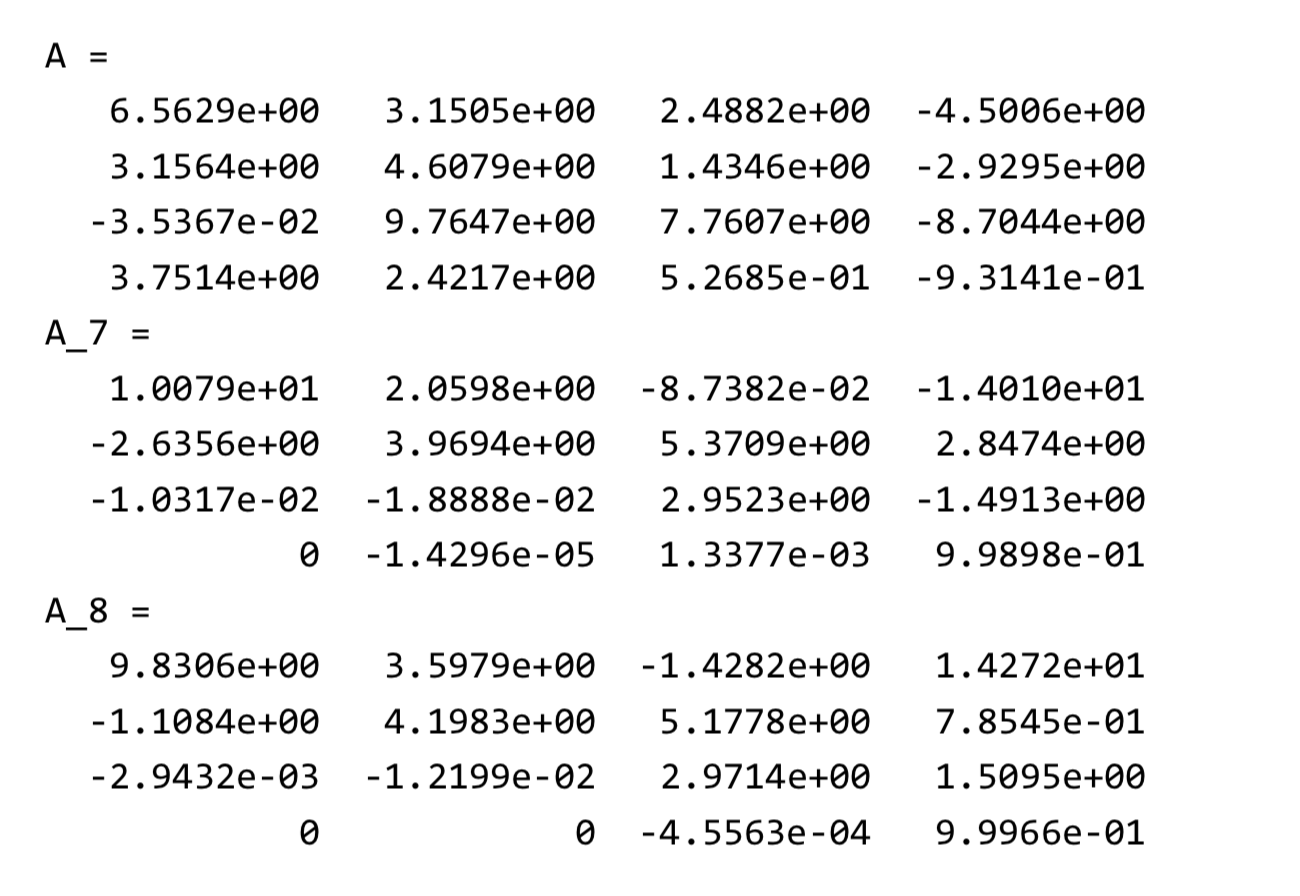
\includegraphics[scale=0.6]{figure4.png}
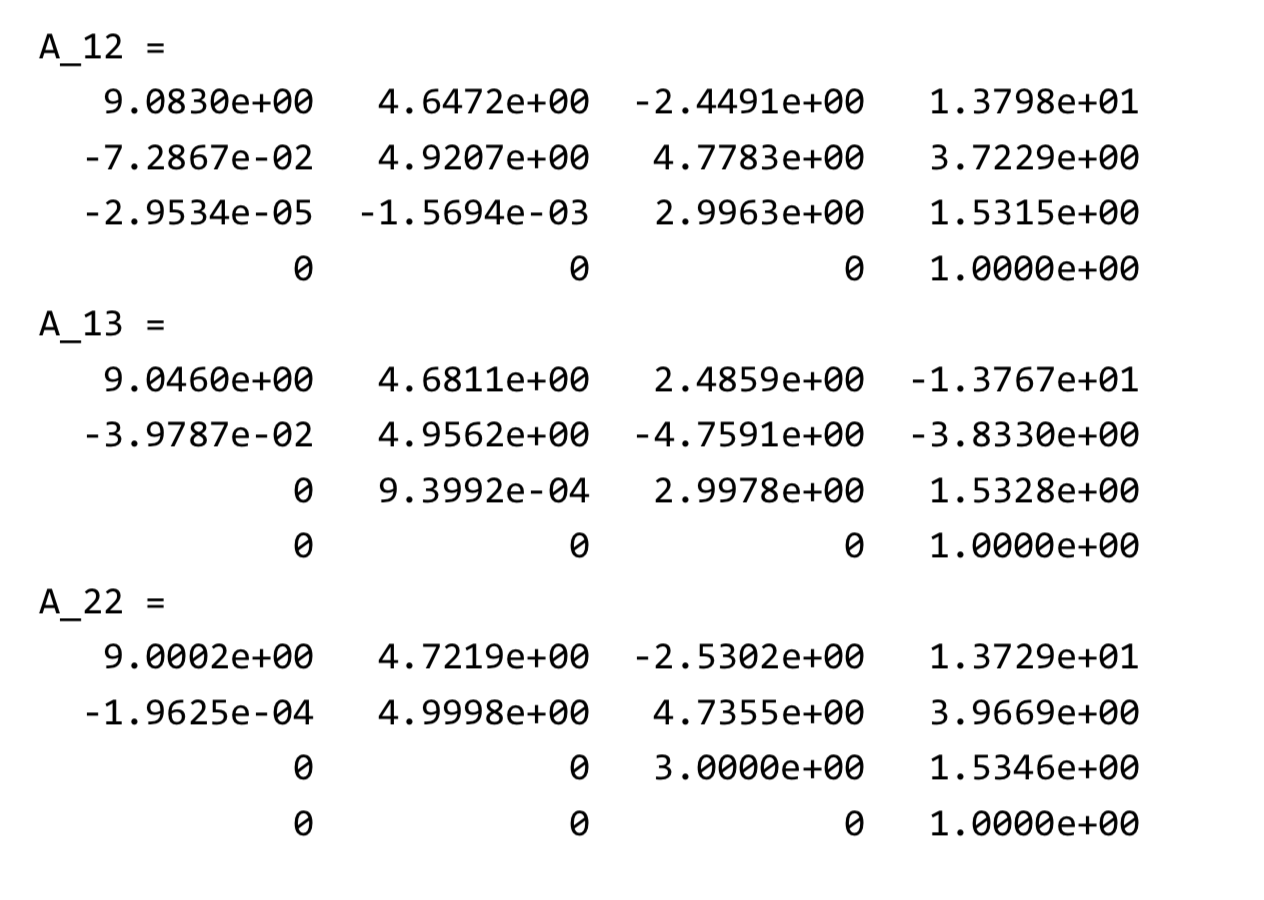
\includegraphics[scale=0.6]{figure5.png}
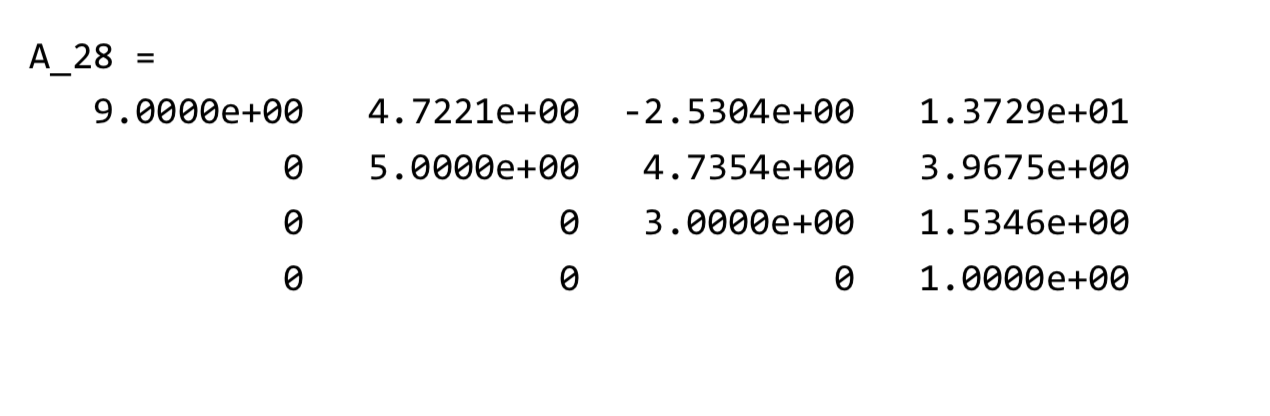
\includegraphics[scale=0.6]{figure6.png}
\end{center}
\end{figure}
\newpage
\subsection{带位移的QR迭代}
为了加快 QR 迭代的收敛速度, 可以采用\textcolor{blue}{位移策略} 和\textcolor{blue}{反迭代}的思想\\
\textcolor{blue}{算法 4.2} 带位移的QR 迭代算法 (QR Iteration with shift)\\
\begin{enumerate}[1:]
\item Set $A_{1}=A$ and $k=1$
\item while not convergence do
\item Choose a shift $\sigma_{k}$
\item \qquad $[Q_{k},R_{k}]=qr(A_{k}-\sigma_{k}I)$
\item \qquad compute $A_{k+1}=R_{k}Q_{k}+\sigma_{k}I$
\item \qquad$k=k+1$
\item end while
\end{enumerate}
正交相似性\\
$$
\begin{aligned} A_{k+1}=R_{k} Q_{k}+\sigma_{k} I &=\left(Q_{k}^{\top} Q_{k}\right) R_{k} Q_{k}+\sigma_{k} I \\ &=Q_{k}^{\top}\left(A_{k}-\sigma_{k} I\right) Q_{k}+\sigma_{k} I \\ &=Q_{k}^{\top} A_{k} Q_{k} \end{aligned}
$$
位移$\sigma_{k}$的选取\\
在前面的分析可知,$A_{k+1}(n, n)$收敛到 A 的模最小特征值.\\
若$\sigma_{k}$就是A的一个特征值,则$A_{k}-\sigma_{k} I$的模最小特征值为0,故QR算 法迭代一步就收敛. 此时
$$
A_{k+1}=R_{k} Q_{k}+\sigma_{k} I=\left[\begin{array}{cc}
{A_{k+1}^{(n-1) \times(n-1)}} & {*} \\
 {0} & {\sigma_{k}}
 \end{array}\right]
$$
A 的其它特征值可通过对$A_{k+1}^{(n-1) \times(n-1)}$使用带位移 QR 迭代算法得到.\\
通常, 如果 $\sigma_{k}$ 与 A 的某个特征值非常接近, 则收敛速度通常会很快. 由 于 $A_{k} (n, n)$ 收敛到 A 的一个特征值, 所以在实际使用中, 一个比较直观 的位移选择策略是$\sigma_{k} =A_{k}(n,n)$.事实上,这样的位移选取方法通常会 使得 QR 迭代算法有二次收敛速度.\\
\\
\textcolor{blue}{例}~带位移的 QR 迭代算法演示 $(见 Eig_QR_shift.m).$\\
所有数据和设置与例 4.1 相同, 在迭代过程中, 取$\sigma_{k}=A_{k}(n, n)$.如果$A_{k}(n, n)$已经收敛, 则取$\sigma_{k}=A_{k}(n-1, n-1)$
\begin{figure}
\begin{center}
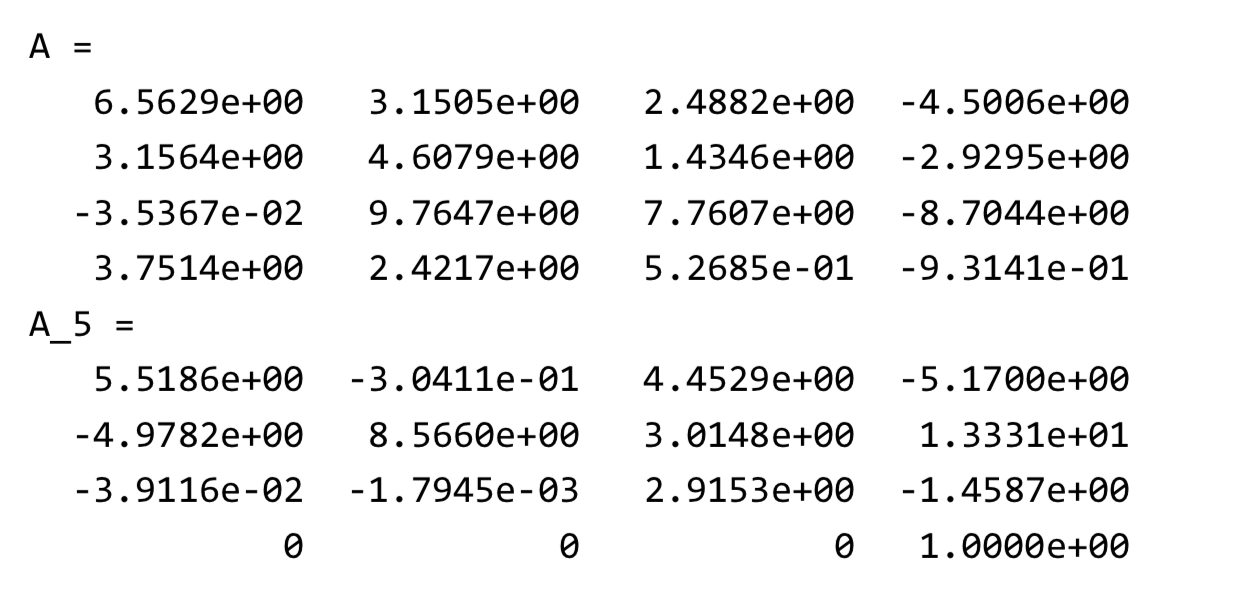
\includegraphics[scale=0.6]{figure7.png}
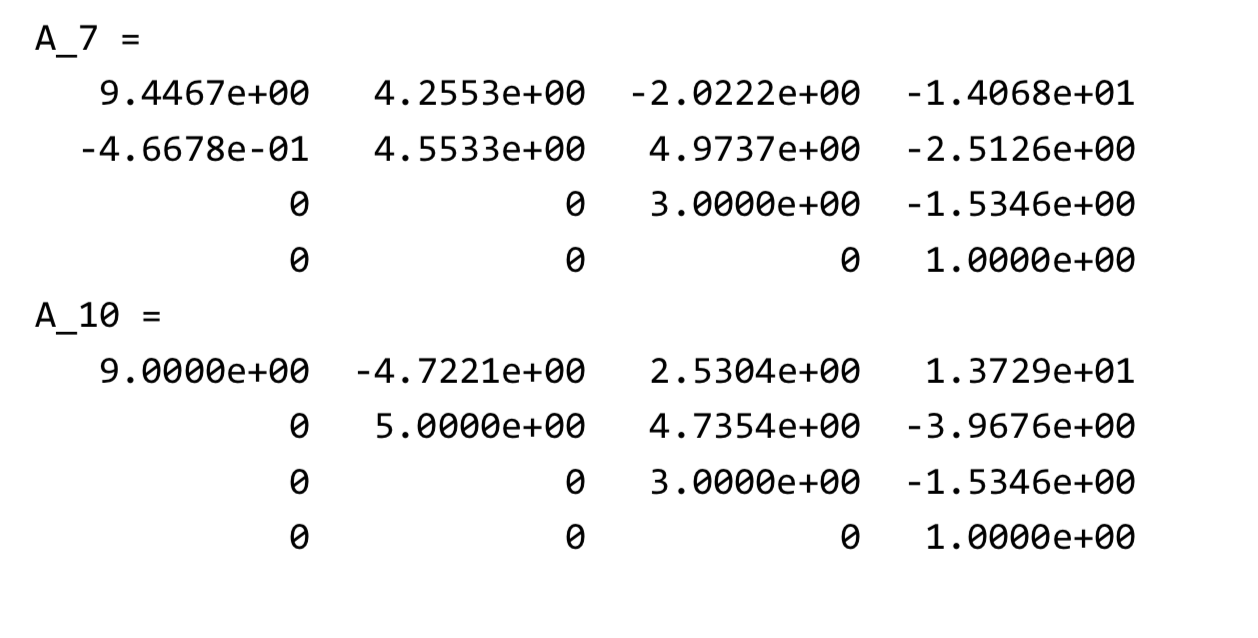
\includegraphics[scale=0.6]{figure8.png}
\end{center}
\end{figure}
\section{带位移的隐式QR迭代}
\noindent \textcolor{blue}{直接实施 QR 方法的困难: 运算量}\\
每一步迭代需要做一次 QR 分解和矩阵乘积, 运算量为 $O\left(n^{3}\right)$ 即使每 计算一个特征值只需迭代一步, 则总运算量为$O\left(n^{4}\right)$\\
我们的目标: 从$O\left(n^{4}\right)$减小到$O\left(n^{3}\right)$\\
实现方法:两个步骤\\
\begin{enumerate}[(1)]
\item 首先通过相似变化将 A 转化成一个 上H
essenberg 矩阵
\item 对这个 Hessenberg 矩阵实施 隐式 QR 迭代
\end{enumerate}
 \textcolor{blue}{隐式 QR 迭代}:\\
 在 QR 迭代算法中, 并 不进行显式的 QR 分解和矩阵乘积 , 而是通过 特殊手段 来实现从$A_{k}$到$A_{k+1}$的迭代,并且将运算量控制在$O\left(n^{2}\right)$量级,从而将总运算量降到$O(n^{3})$
\subsection{上 Hessenberg 矩阵}
 \noindent \textcolor{blue}{上Hessenberg矩阵:}$H=\left[h_{i j}\right] \in \mathbb{R}^{n \times n}$当$i>j+1$时,有$h_{i j}=0$\\
 \textcolor{blue}{定理}设$A \in \mathbb{R}^{n \times n}$,则存在正交矩阵$Q \in \mathbb{R}^{n \times n}$使得$Q A Q^{\top}$是上Hessenberg矩阵\\
 下面我们以一个 $5\times 5$ 的矩阵 A 为例, 给出具体的转化过程, 采用的工具 为 Householder 变换.\\
\textcolor{blue}{第一步}:令$Q_{1}=\operatorname{diag}\left(I_{1 \times 1}, H_{1}\right)$,其中$H_{1}$是对应于向量$A(2 : 5,1)$的 Householder 矩阵. 于是可得
$$
Q_{1} A=\left[\begin{array}{ccccc}
* &*& *& *&* \\ 
* &*& *& *&* \\ 
0 &*& *& *&*\\ 
0 &*& *& *&*\\ 
0 &*& *& *&*
\end{array}\right]
$$
由于用$Q_{1}^{T}$右乘$Q_{1} A$,不会改变$Q_{1} A$的第一列元素的值,故
$$
A_{1} \triangleq Q_{1} A Q_{1}^{\top}=\left[\begin{array}{ccccc}
* &*& *& *&* \\ 
* &*& *& *&* \\ 
0 &*& *& *&*\\ 
0 &*& *& *&*\\ 
0 &*& *& *&*
\end{array}\right]
$$
\textcolor{blue}{第二步}:令$Q_{2}=\operatorname{diag}\left(I_{2 \times 2}, H_{2}\right)$,其中$H_{2}$是对应于向量$A_{1}(3 : 5,2)$的 Householder 矩阵, 则用 $Q_{2}$ 左乘 $A_{1} $时, 不会改变 $A_{1}$ 的第一列元素 的值. 用$Q_{2}^{\top}$右乘$Q_{2} A_{1}$时,不会改变$Q_{2} A_{1}$前两列元素的值.因此
$$
Q_{2} A_{1}=\left[\begin{array}{ccccc}
* &*& *& *&* \\ 
* &*& *& *&* \\ 
0 &*& *& *&*\\ 
0 &0& *& *&*\\ 
0 &0& *& *&*
\end{array}\right]和
A_{2}\triangleq Q_{2} A_{1} Q_{2}^{\top}=\left[\begin{array}{ccccc}
* &*& *& *&* \\ 
* &*& *& *&* \\ 
0 &*& *& *&*\\ 
0 &0& *& *&*\\ 
0 &0& *& *&*
\end{array}\right]
$$
\textcolor{blue}{第三步}:
令$Q_{3}=\operatorname{diag}\left(I_{3 \times 3}, H_{3}\right)$,其中$H_{3}$是对应于向量$A_{2}(4 : 5,3)$的Householder 矩阵, 则有
$$
Q_{3} A_{2}=\left[\begin{array}{ccccc}
* &*& *& *&* \\ 
* &*& *& *&* \\ 
0 &*& *& *&*\\ 
0 &0& *& *&*\\ 
0 &0& 0& *&*
\end{array}\right]和A_{3} \triangleq Q_{3} A_{2} Q_{3}^{\top}=\left[\begin{array}{ccccc}
* &*& *& *&* \\ 
* &*& *& *&* \\ 
0 &*& *& *&*\\ 
0 &0& *& *&*\\ 
0 &0& 0& *&*
\end{array}\right]
$$
这时我们就将A转化成一个上Hessenberg矩阵,即
$Q A Q^{\top}=A_{3}$,其中$Q=Q_{3} Q_{2} Q_{1}$是正交矩阵,$A_{3}$是上Hessenberg矩阵.


\end{document}